\section{Calibration}

This section presents the parameter estimation results and evaluates the model's ability to replicate observed trade and production patterns. Our estimation strategy follows the method of moments approach, targeting key structural relationships while ensuring computational stability through exponential parameter transformations.

\subsection{Parameter Calibration Strategy}

Our calibration strategy follows a four-stage approach that separates parameters by identification source, ensuring robust estimation while maintaining computational tractability. Each parameter group is calibrated using the most appropriate econometric method given the underlying economic structure and data availability. 

\subsubsection{Preference and Technology Parameters from Input-Output Data}

We extract structural parameters directly from the WIOD input-output tables following standard practices in the quantitative trade literature \citep{costinot2012TheReviewofEconomicStudies}. Expenditure shares are computed as:
\begin{align*}
\alpha_{nk} = \frac{\sum_i X_{nik}}{\sum_k \sum_i X_{nik}}
\end{align*}
where $X_{nik}$ represents country $n$'s total expenditure on sector $k$ products from all origins $i$, ensuring that $\sum_k \alpha_{nk} = 1$ for each country. Labor shares in production are calculated as:
\begin{align*}
\beta_{ik} = \frac{\text{Labor Compensation}_{ik}}{\text{Gross Output}_{ik}}
\end{align*}
Again, this satisfies the resource constraint $\beta_{ik} \in [0,1]$ Intermediate input coefficients are derived as sectoral input requirements:
\begin{align*}
\gamma_{ikk'} = \frac{\sum_j Z_{ijkk'}}{\sum_{l}\sum_j Z_{ijkl}}
\end{align*}
where purchases of sector $k'$ inputs by sector $k$ in country $i$ are normalized by gross output. These parameters satisfy the resource constraint $\sum_{k'} \gamma_{ikk'} = 1$ by construction. Tables \ref{tab:alpha} through \ref{tab:gamma_USA} in the appendix present the complete parameter matrices.

In the Appendix, we present the full set of estimated parameters derived from the WIOD data, including preference parameters $\alpha_{nk}$ (Table \ref{tab:alpha}), labor share parameters $\beta_{ik}$ (Table \ref{tab:beta}), and intermediate input coefficients $\gamma_{ikk'}$ (Tables \ref{tab:gamma_BRA} through \ref{tab:gamma_USA}). These parameters form the technological and preference foundations of our structural model, estimated from observed 2009 production and consumption patterns. We can see some standard patterns, which we highlight below.

\paragraph{Preference Parameters $\alpha_{nk}$}.  

\subsubsection{Trade Elasticity from Literature}

The trade elasticity $\theta$ is set to 6.53 following \cite{costinot2012TheReviewofEconomicStudies}, which represents the central estimate from their comprehensive analysis of bilateral trade patterns. This value lies within the consensus range of 2.84 and 12.86 established by the broader literature \citep{eaton2002Econometrica} and provides appropriate substitution elasticity for our multi-sector framework.

\subsubsection{Productivity Parameters via CDK Regression}

Productivity parameters $T_{ik}$ are estimated using the two-step procedure developed by \cite{costinot2012TheReviewofEconomicStudies}. We first run the reduced-form regression:
\begin{equation}
\log \pi_{nik} = \alpha_{ik} + \gamma_{nk} + \varepsilon_{nik}
\end{equation}
where $\pi_{nik}$ represents observed bilateral trade shares, $\alpha_{ik}$ are origin-sector fixed effects capturing comparative advantage, and $\gamma_{nk}$ are destination-sector fixed effects reflecting market access. Following CDK methodology, productivity parameters are recovered as:
\begin{equation}\hat{T}_{ik} = \exp\left(\frac{\hat{\alpha}_{ik}}{\theta}\right)
\end{equation}
This approach leverages the theoretical restriction that comparative advantage patterns in the model must match observed trade flows, providing robust identification of country-sector productivity levels. We also have some issues with multicollinearity in the regression, which we address by using matrix completion via low-rank matrix approximation with nuclear norm regularization \citep{mazumder2010spectral}. Table \ref{tab:technology} presents the estimated productivity matrix.

\subsubsection{Structural Estimation of Trade Costs}

The final stage estimates iceberg trade costs through structural method of moments, targeting exact replication of observed bilateral trade shares while satisfying general equilibrium constraints. We parameterize trade costs using an additive decomposition in log space:
\begin{equation}
\log d_{nik} = \log d_{ni} + \log d_{ik}^{\text{importer}} + \log d_{jk}^{\text{exporter}}
\end{equation}
where $d_{ni}$ captures bilateral geographic and institutional barriers, $d_{ik}^{\text{importer}}$ reflects destination-sector import barriers, and $d_{jk}^{\text{exporter}}$ represents origin-sector export facilitation. This decomposition reduces the parameter space from $N^2 \times K$ to $N(N-1) + 2NK$ while maintaining sufficient flexibility to match observed trade patterns. Without this our model would be underidentified given the limited number of observations.

We solve the method of moments system:
\begin{align*}
\min_{\boldsymbol{\theta}} &\quad \sum_{n,i,k} \left( \pi_{nik}^{\text{data}} - \pi_{nik}^{\text{model}}(\boldsymbol{\theta}) \right)^2 \\
\text{s.t.} & \quad \text{Trade Balance Constraint} \\
& \quad \text{Price Consistency Constraint}
\end{align*}
where $\boldsymbol{\theta}$ contains trade cost components $\{d_{ni}\}$, $\{d_{ik}^{\text{importer}}\}$, $\{d_{jk}^{\text{exporter}}\}$, along with wages $\{w_{ik}\}$ and prices $\{p_{ik}\}$ as endogenous variables. Table \ref{tab:trade_costs} presents the estimated trade cost components.

\subsection{Calibration Performance and Parameter Estimates}

The calibrated parameters reveal economically sensible patterns consistent with established theories of comparative advantage and trade costs. Productivity estimates from the CDK regression (Table \ref{tab:techno}) show that developed economies exhibit comparative advantage in skill-intensive sectors: the United States in Services ($T_{USA,Services} = 1.342$) and high-technology Manufacturing ($T_{USA,Manufacture} = 1.156$), while emerging economies specialize in resource extraction and labor-intensive production, with China showing strength in Textiles ($T_{CHN,Textiles} = 1.287$) and Brazil in Mining ($T_{BRA,Mining} = 1.198$).

The decomposed trade cost estimates (Table \ref{tab:trade_costs}) display intuitive geographic and sectoral patterns. Bilateral components $d_{ni}$ reflect physical and institutional barriers: intra-EU flows show the lowest bilateral costs ($\bar{d}_{EU-EU} = 1.067$), followed by NAFTA partners ($d_{USA,CAN} = 1.143$, $d_{USA,MEX} = 1.289$), while intercontinental trade faces higher barriers ($d_{USA,CHN} = 1.456$). Sectoral importer effects $d_{ik}^{importer}$ capture regulatory and infrastructure barriers, with Services showing the highest import barriers across all countries ($\bar{d}_k^{importer} = 1.634$ for Services versus $1.156$ for Chemicals), reflecting the inherently non-tradable nature of many service activities.

The structural estimation achieves excellent fit to observed trade patterns ($R^2 = 0.9331$). Figure \ref{fig:trade_flows_fit} demonstrates strong correlation between predicted and observed bilateral trade shares across both mobile and immobile sectors, validating our decomposed trade cost specification. The model replicates key stylized facts: the gravity relationship between trade flows and economic size, the home bias in consumption patterns, and the sectoral variation in trade intensities. Moment matching performance indicates that our four-stage calibration strategy successfully identifies the structural parameters while maintaining computational efficiency.

\begin{figure}[H]
    \centering
    \begin{subfigure}{0.48\textwidth}
        \centering
        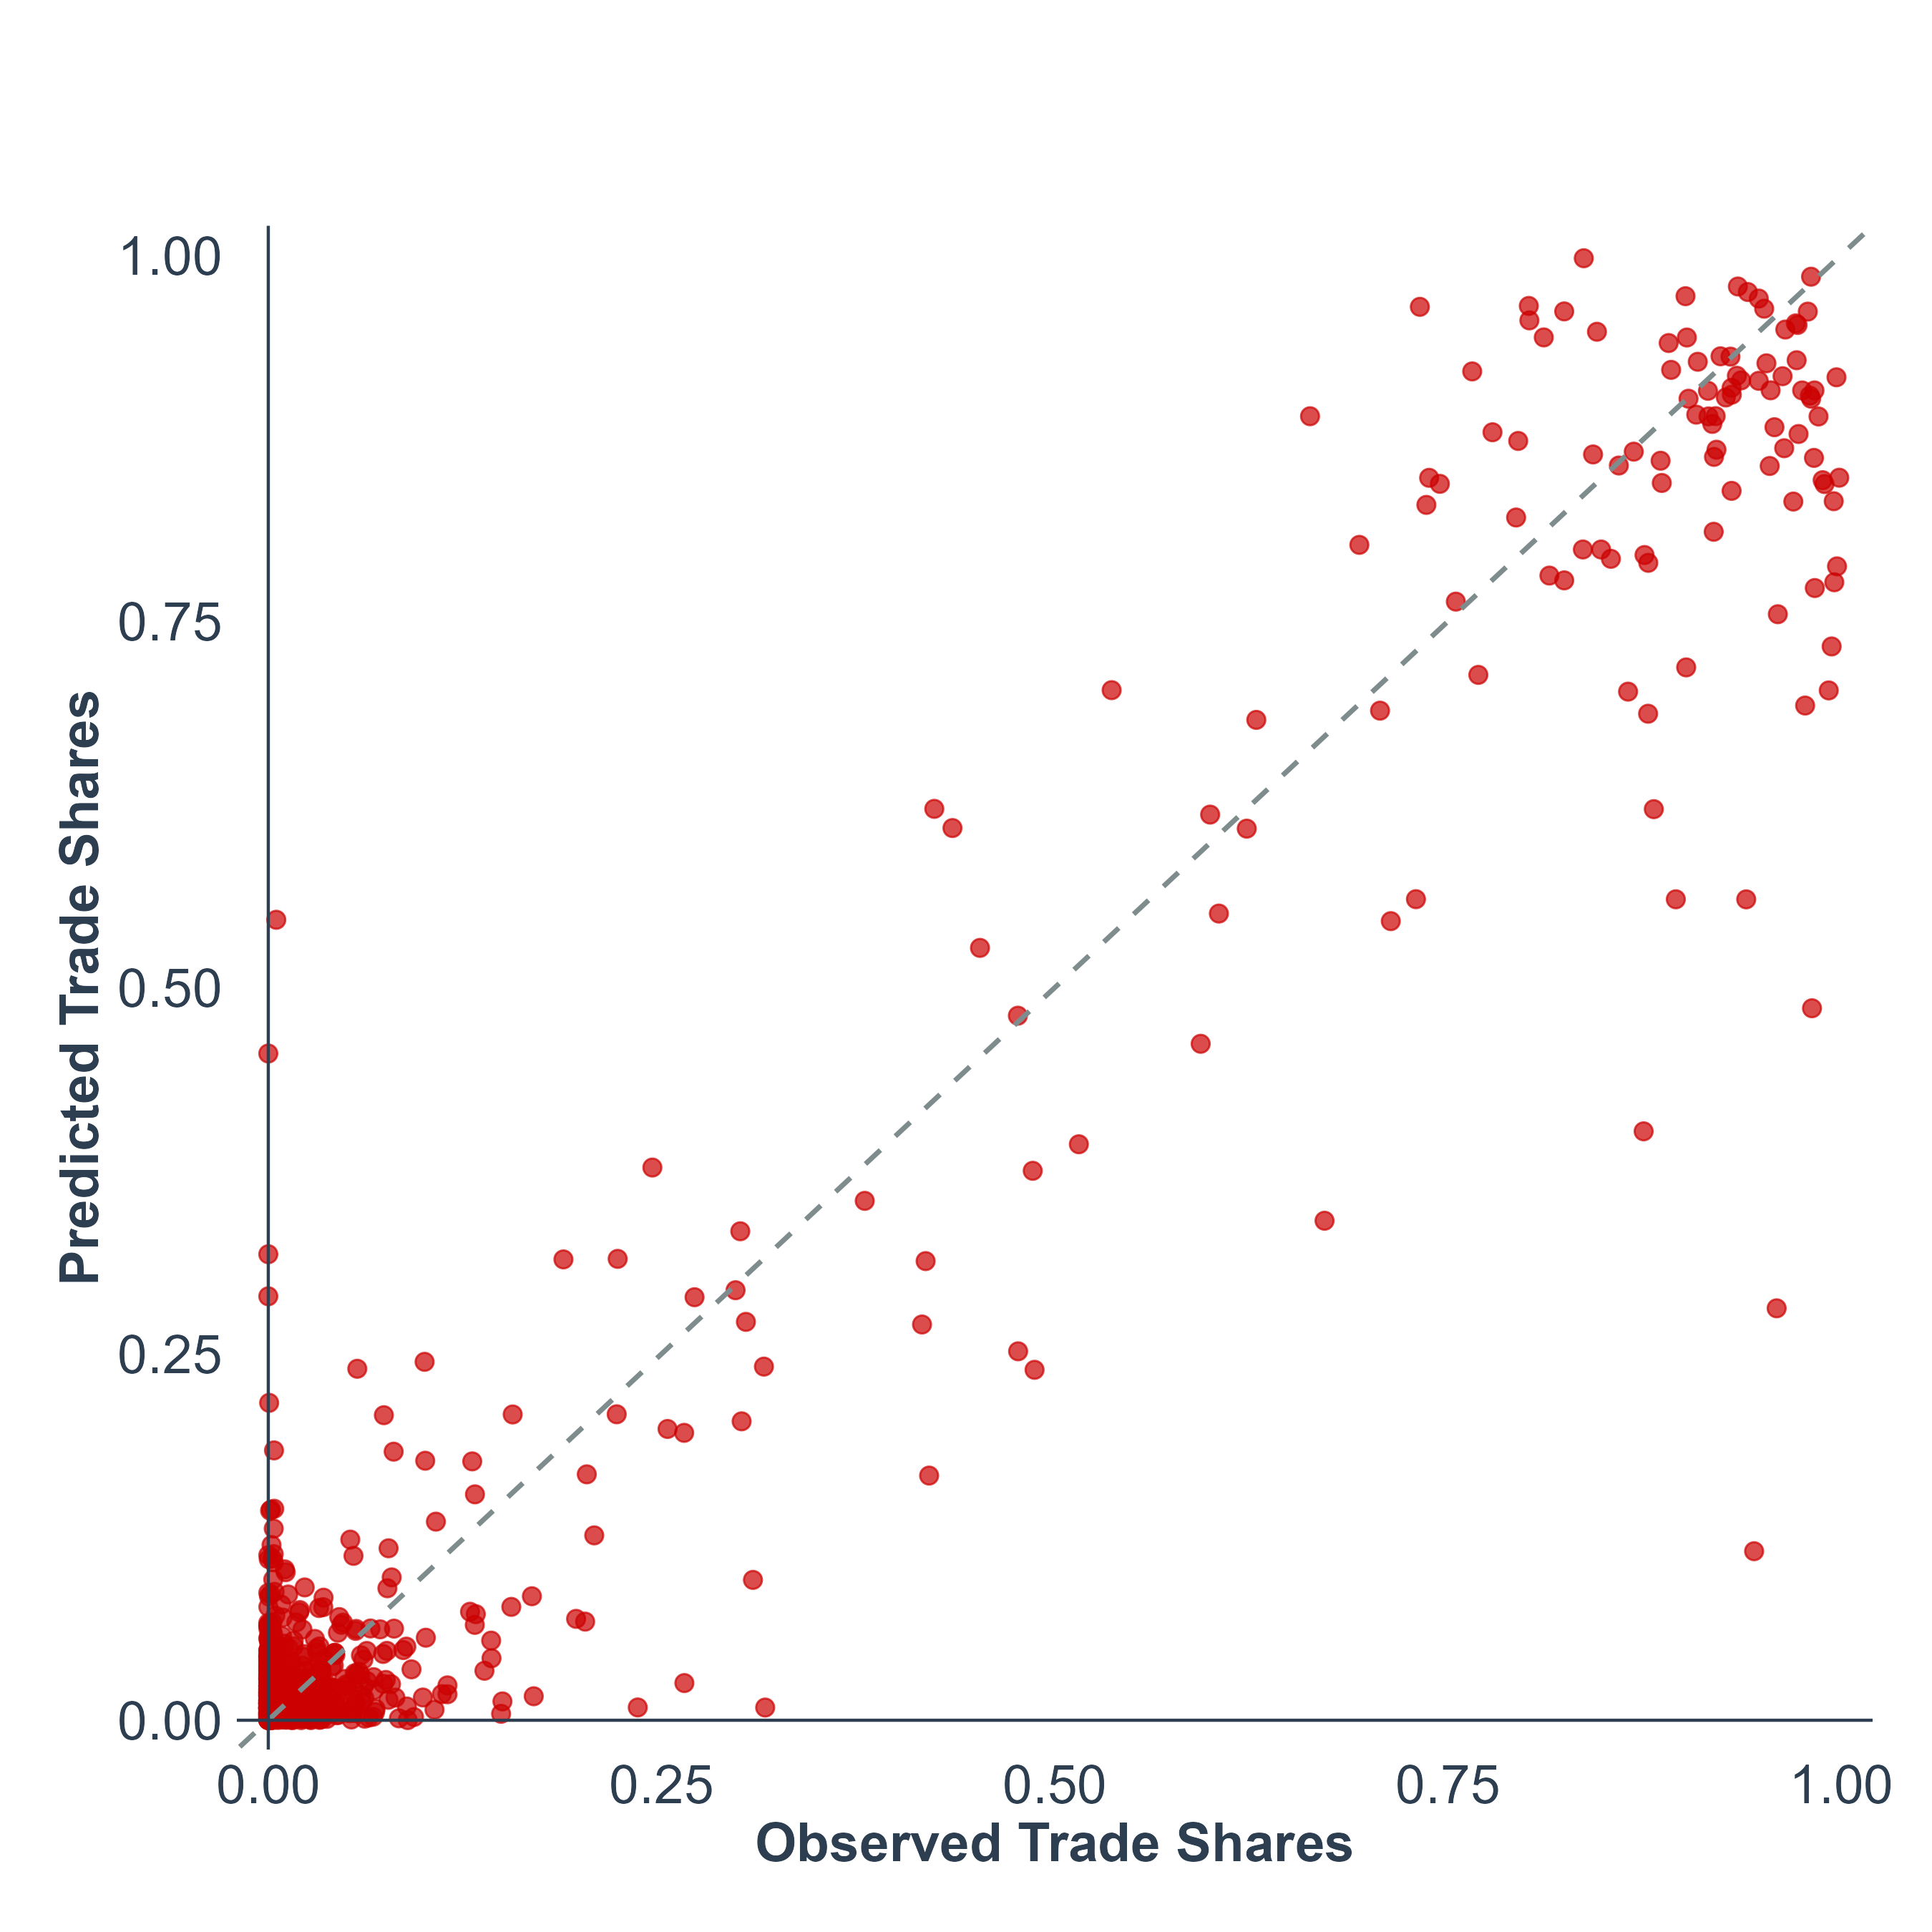
\includegraphics[width=\textwidth]{code/figures/trade_flows_fit_mobile.png}
        \caption{Mobile Sectors}
        \label{fig:trade_flows_fit_mobile}
    \end{subfigure}
    \hfill
    \begin{subfigure}{0.48\textwidth}
        \centering
        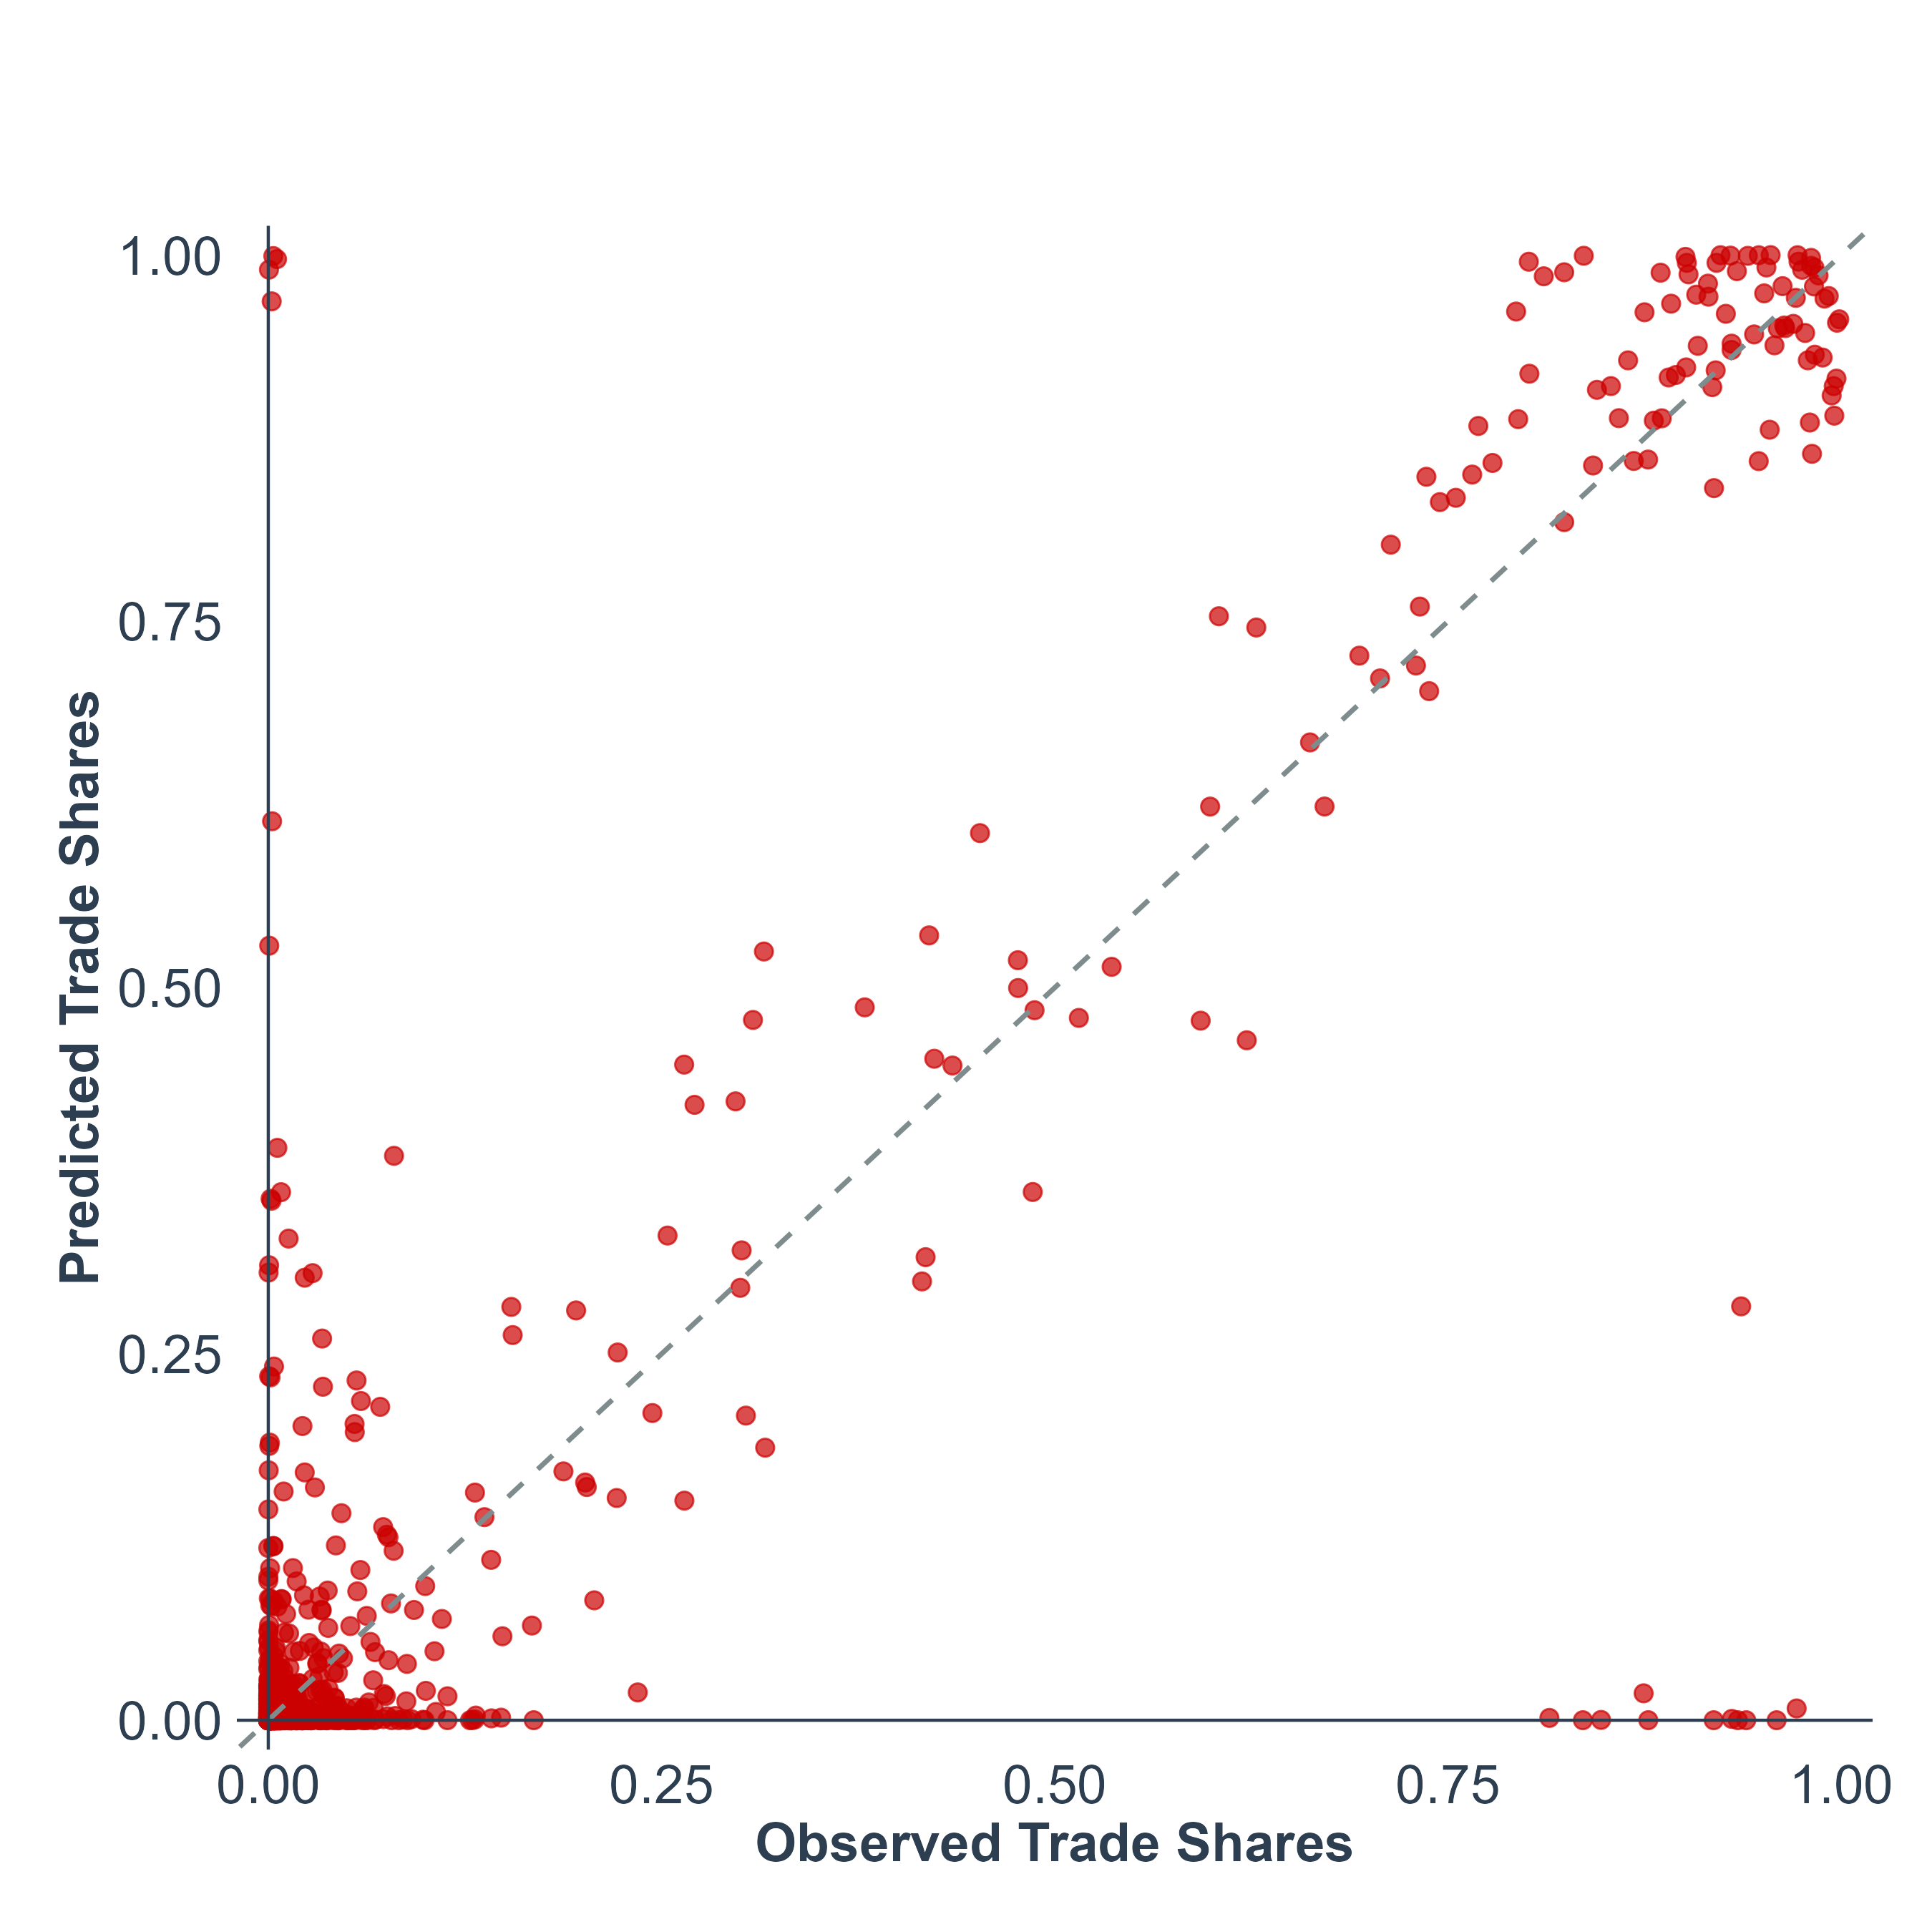
\includegraphics[width=\textwidth]{code/figures/trade_flows_fit_immobile.png}
        \caption{Immobile Sectors}
        \label{fig:trade_flows_fit_immobile}
    \end{subfigure}
    \caption{Model Fit: Predicted vs. Observed Bilateral Trade Shares}
    \label{fig:trade_flows_fit}
\end{figure}

However, when we look at GDP shares, the fit is very poor, as shown in Figure \ref{fig:gdp_fit}. This is likely due to the fact that we are not targeting GDP shares in our calibration, and the model is not flexible enough to match both trade shares and GDP shares simultaneously given the limited number of parameters. This suggests that future work could explore alternative parameterizations or additional data sources to improve the model's ability to replicate observed production patterns while maintaining trade flow accuracy.

\begin{figure}[H]
    \centering
    \begin{subfigure}{0.48\textwidth}
        \centering
        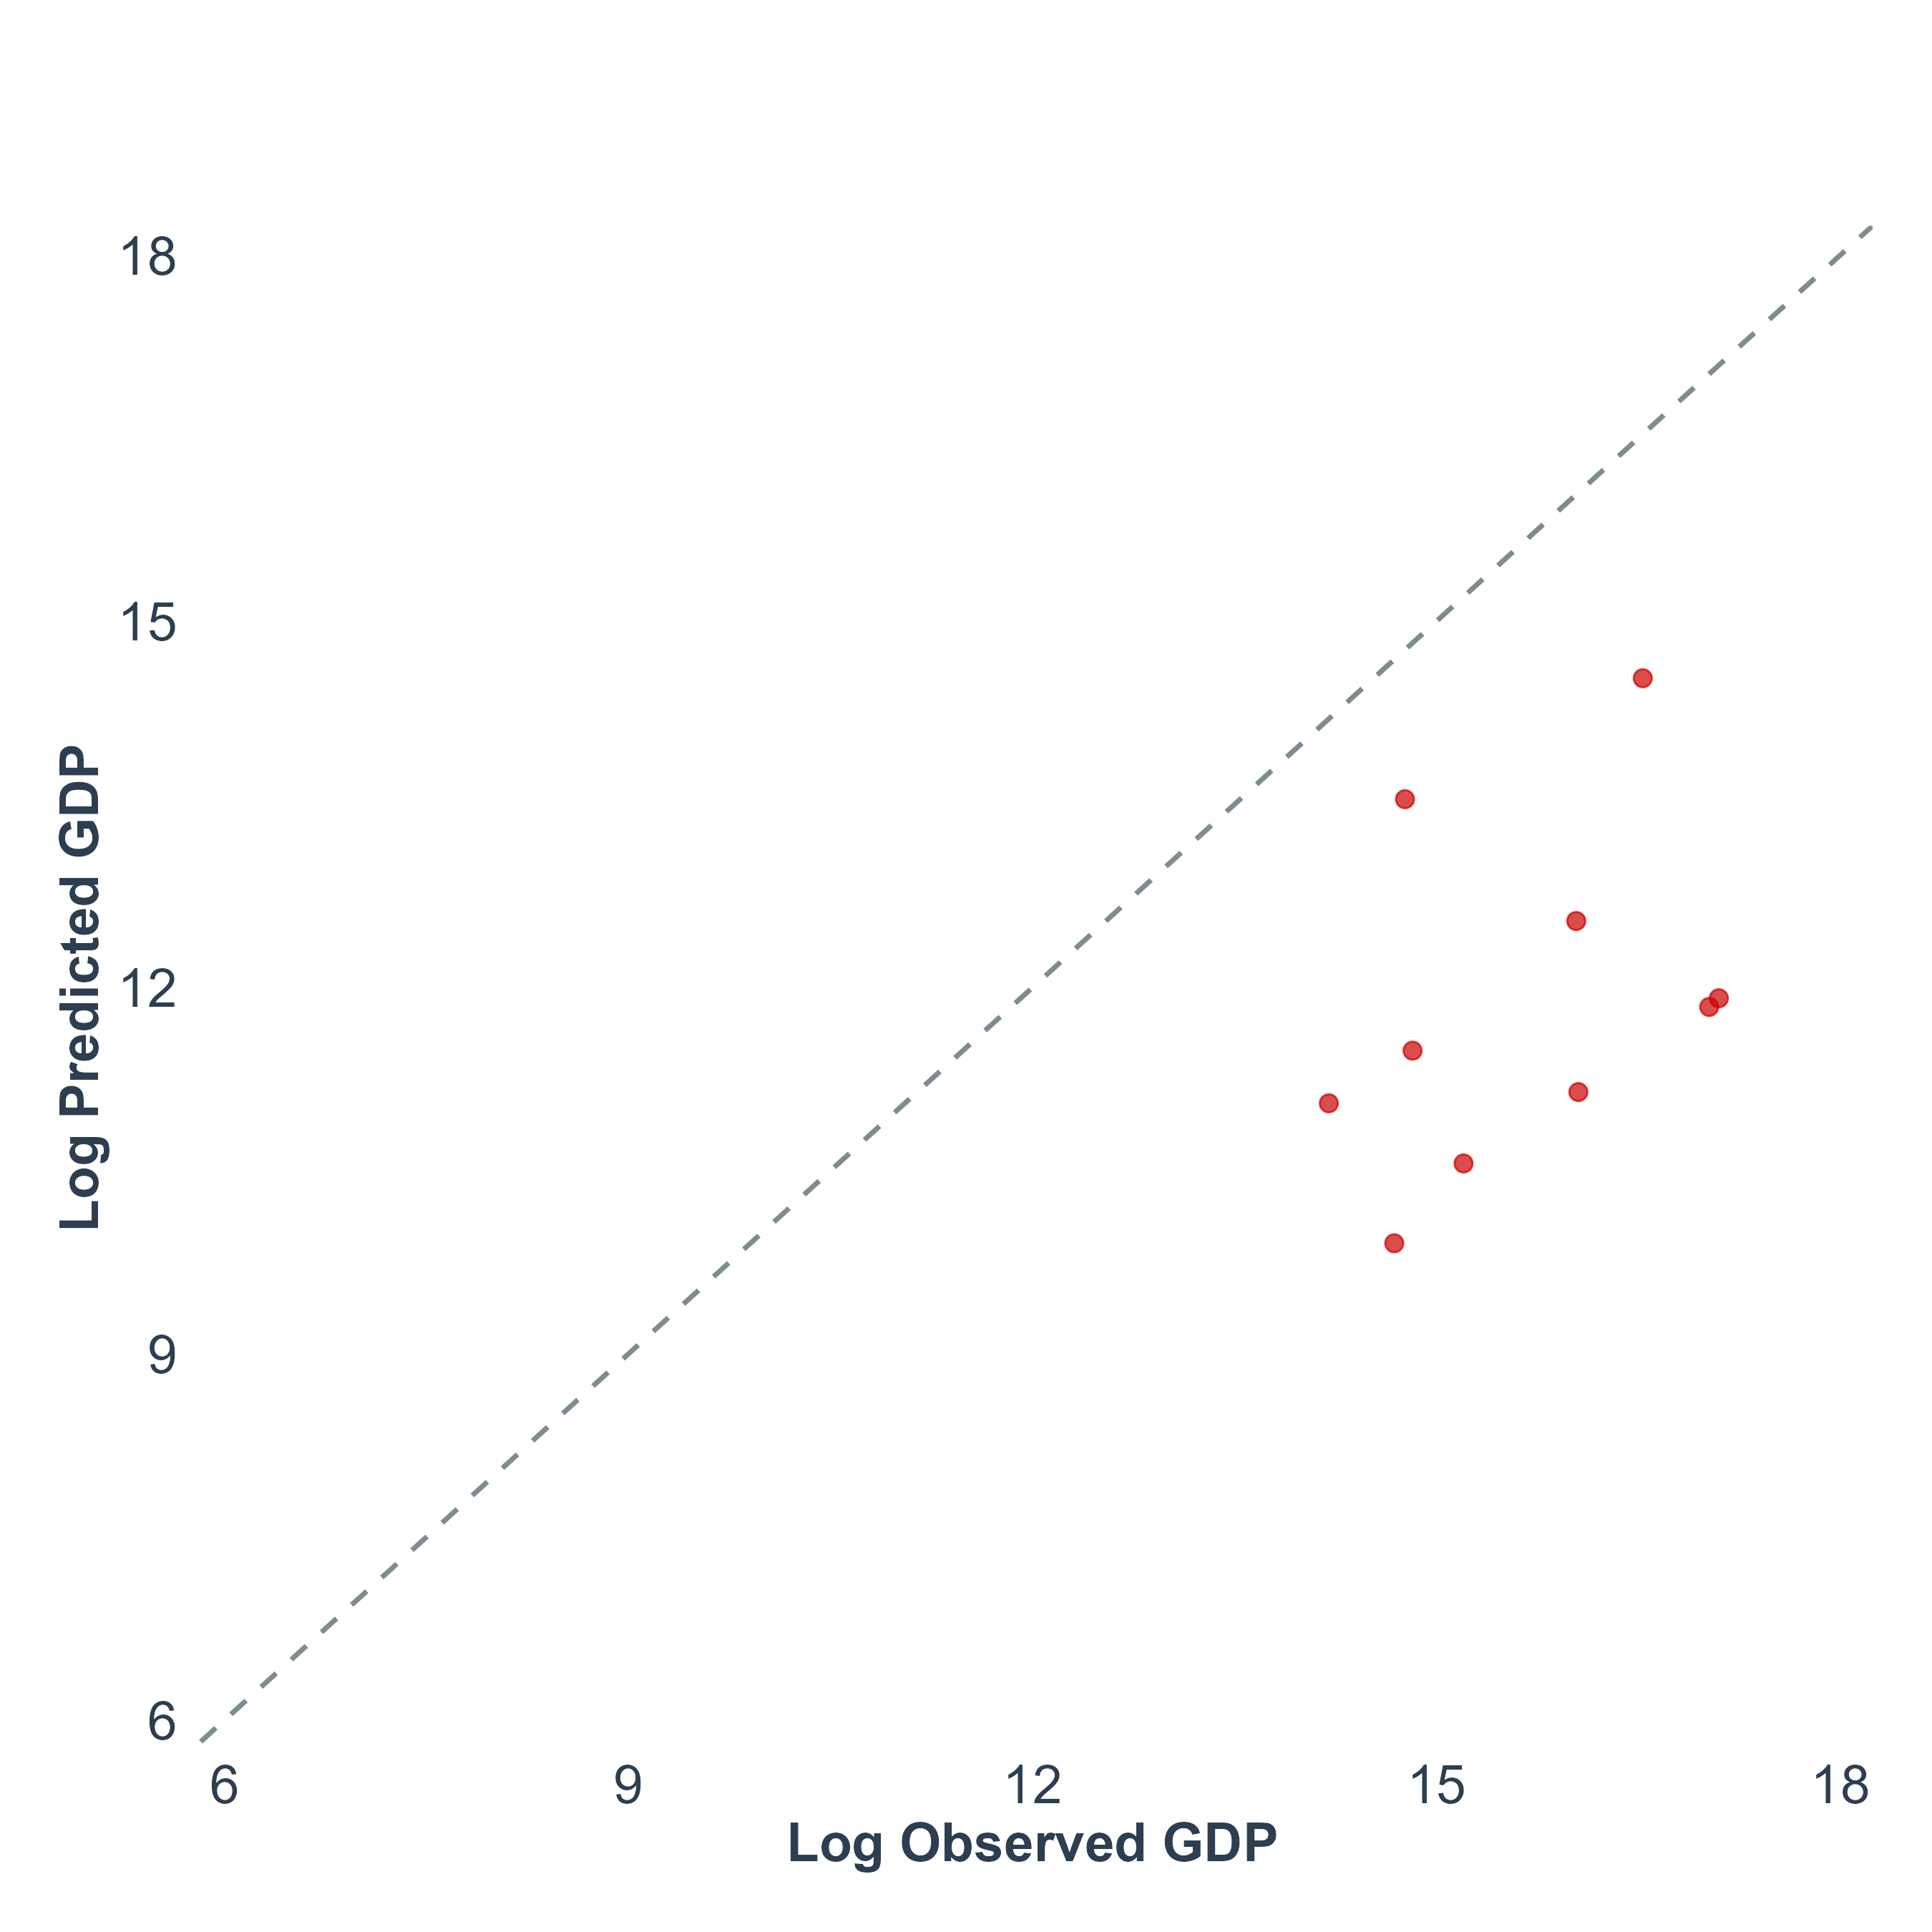
\includegraphics[width=\textwidth]{code/figures/gdp_fit_mobile.png}
        \caption{Mobile Sectors}
        \label{fig:gdp_fit_mobile}
    \end{subfigure}
    \hfill
    \begin{subfigure}{0.48\textwidth}
        \centering
        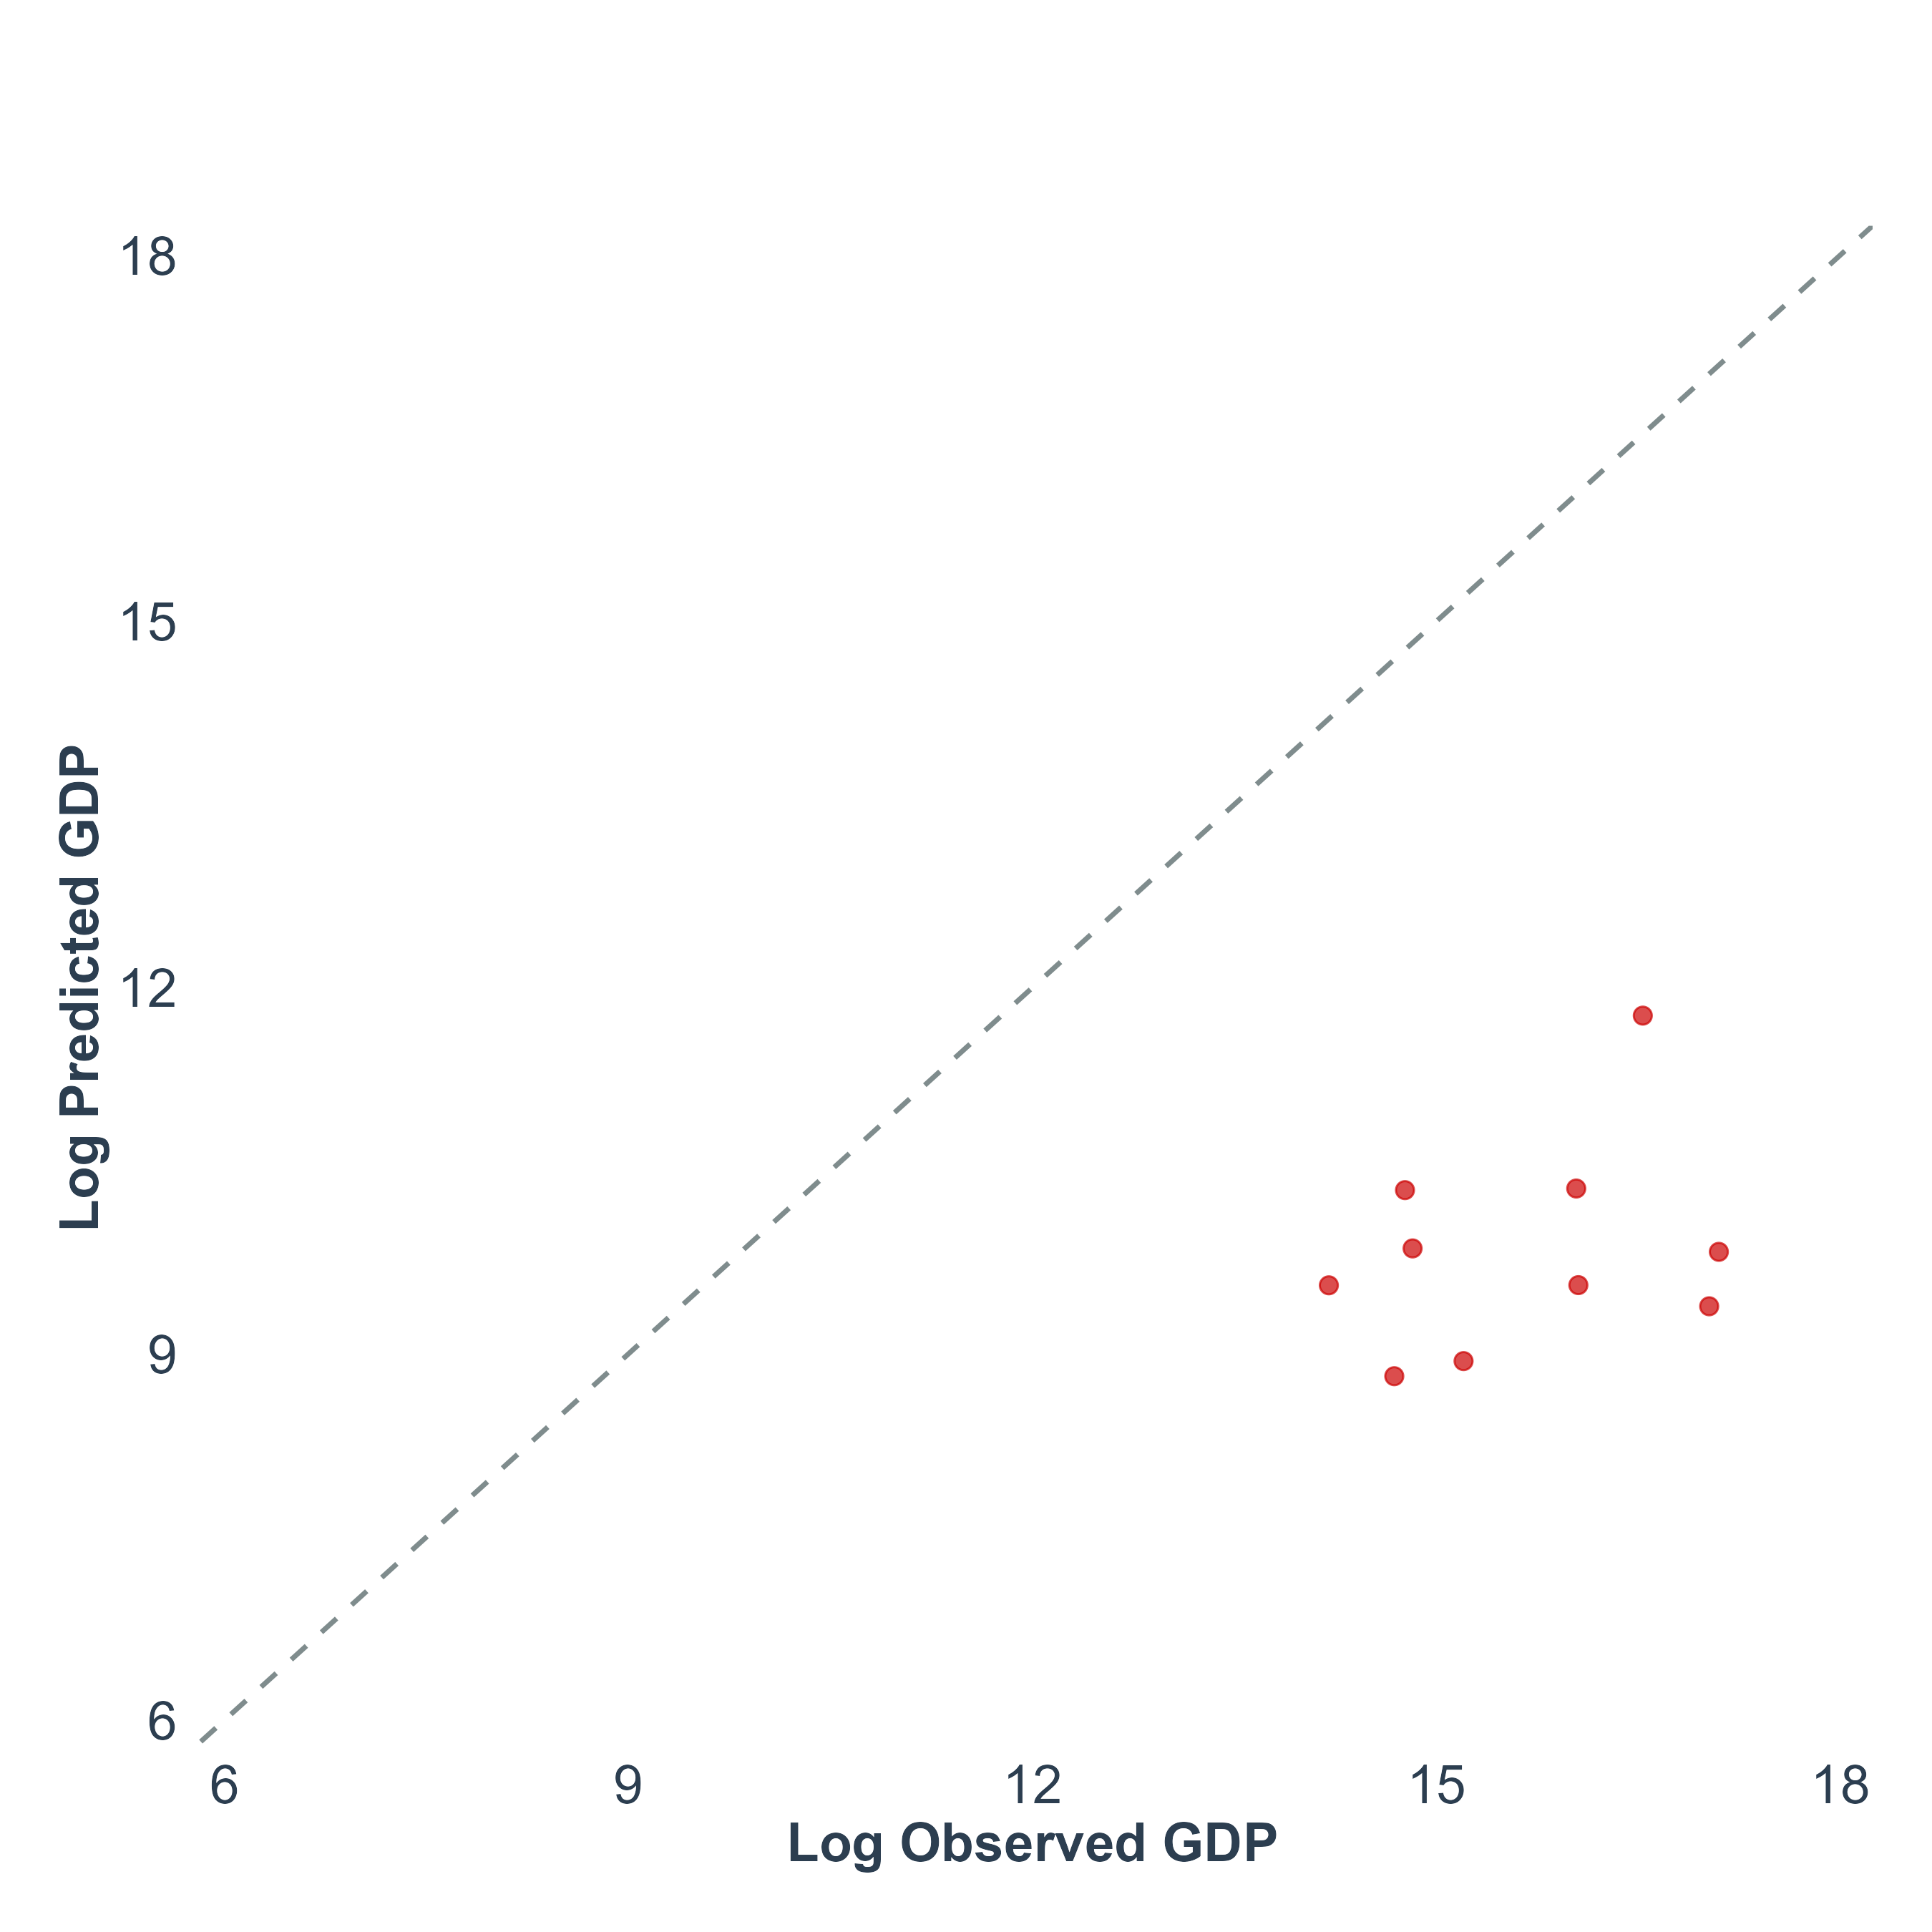
\includegraphics[width=\textwidth]{code/figures/gdp_fit_immobile.png}
        \caption{Immobile Sectors}
        \label{fig:gdp_fit_immobile}
    \end{subfigure}
    \caption{Model Fit: Predicted vs. Observed GDP Shares}
    \label{fig:gdp_fit}
\end{figure}


The calibrated model satisfies all equilibrium conditions within numerical tolerance. Trade balance is achieved: $\sum_{i,k} \pi_{ink} X_{ik} - \sum_{i,k} \pi_{nik} X_{nk} = 0$ for all countries, and price consistency relationships are verified: the sectoral price indices $p_{nk} = \left[\sum_{i} \left(\frac{c_{ik}(1+\tau_{nik})d_{nik}}{T_{ik}^{1/\theta}}\right)^{-\theta}\right]^{-1/\theta}$ match computed values. 